\begin{exercise}
The results shown in Figure \ref{fig:1.6} (below) should be quite reliable because they are averages over $2000$ individual, randomly chosen $10$-armed bandit tasks.
Why, then, are there oscillations and spikes in the early part of the curve for the optimistic method?
In other words, what might make this method perform particularly better or worse, on average, on particular early steps?

\begin{figure}[H]
    \centering
    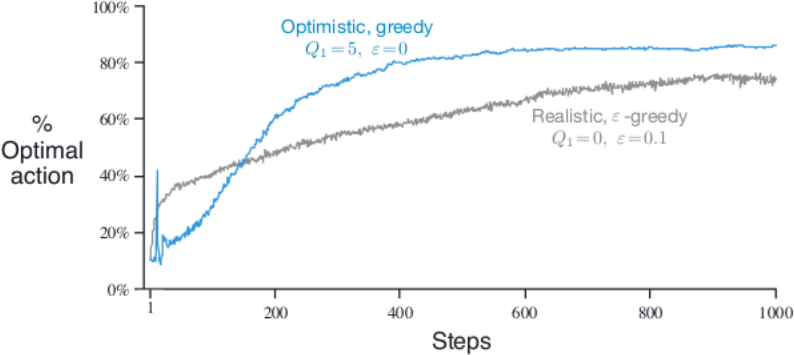
\includegraphics[width = 0.5 \textwidth]{1.6.png}
    \caption
    {
        The effect of optimistic initial action-value estimates on the $10$-armed testbed.
        Both methods used a constant step-size parameter, $\alpha = 0.1$.
    }
    \label{fig:1.6}
\end{figure}
\end{exercise}

\begin{solution}
Because of the optimistic initial action-value estimates we need to do a \"downwards-correction\" of the action-value estimates. So in the first 10 steps it is almost guaranteed that every action is taken once and since the action-value estimate is going to be lowered we are taking another action where the action-value estimate is still $5$. After the first round of corrections we take the optimal action with increased likelyhood, since it is likely reduced by the smallest amount (because we likely get the highest reward). So the peak is probably in step $11$. Since the action-value estimates are still too high after the first round of corrections, a second downwards-correction for all actions has to be done. So we have likely taken the optimal action in step $11$ (or maybe $12$ if some action yields similar high rewards) but now we take all other actions again to finish the downwards-correction of our action-value estimates. So in the next few steps the likelyhood of taking the optimal action is decreased.
\end{solution}
